\documentclass[tikz,border=4pt]{standalone}
\usepackage{xcolor}
\usetikzlibrary{arrows.meta, positioning}
\definecolor{edgeblue}{HTML}{2F6FED}
\definecolor{edgegreen}{HTML}{2E8B57}
\definecolor{edgeorange}{HTML}{D9822B}
\definecolor{edgegray}{HTML}{F2F4F8}
\begin{document}
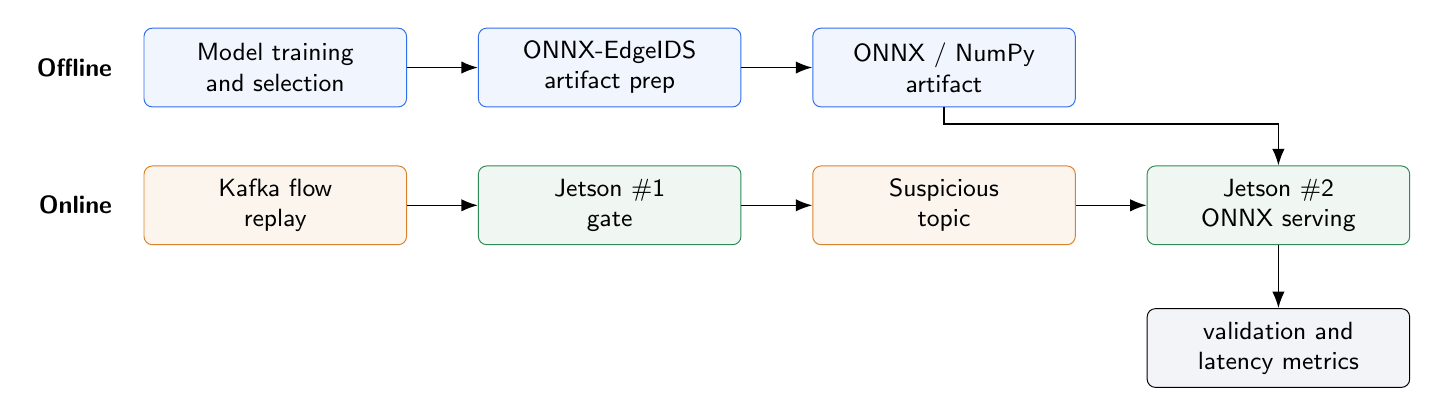
\begin{tikzpicture}[
  node distance=8mm and 9mm,
  stage/.style={draw, rounded corners=3pt, align=center, minimum height=10mm,
    text width=31mm, fill=edgegray, line width=0.35pt, font=\sffamily\small},
  blue/.style={stage, draw=edgeblue, fill=edgeblue!7},
  green/.style={stage, draw=edgegreen, fill=edgegreen!7},
  orange/.style={stage, draw=edgeorange, fill=edgeorange!8},
  arrow/.style={-{Latex[length=2.1mm]}, line width=0.55pt},
  lane/.style={font=\sffamily\bfseries\small, anchor=east}
]
\node[blue] (train) at (0, 0) {Model training\\and selection};
\node[blue, right=of train] (exporter) {ONNX-EdgeIDS\\artifact prep};
\node[blue, right=of exporter] (artifact) {ONNX / NumPy\\artifact};

\node[orange] (replay) at (0, -1.75) {Kafka flow\\replay};
\node[green, right=of replay] (gate) {Jetson \#1\\gate};
\node[orange, right=of gate] (topic) {Suspicious\\topic};
\node[green, right=of topic] (serve) {Jetson \#2\\ONNX serving};

\node[stage, below=8mm of serve, text width=31mm] (metrics) {validation and\\latency metrics};

\draw[arrow] (train) -- (exporter);
\draw[arrow] (exporter) -- (artifact);
\draw[arrow] (artifact) -- ++(0,-0.72) -| (serve);
\draw[arrow] (replay) -- (gate);
\draw[arrow] (gate) -- (topic);
\draw[arrow] (topic) -- (serve);
\draw[arrow] (serve) -- (metrics);
\node[lane] at (-1.95, 0) {Offline};
\node[lane] at (-1.95, -1.75) {Online};
\end{tikzpicture}
\end{document}
